\subsection{Gaussian Mixture Model (GMM)}

\textbf{Problems and compensations}: As explained in report 1, the ratio attributes in the data matrix $\bm{X}$ were standardized by subtracting the estimated mean $\hat{\mu}$ and dividing with the estimated standard deviation $\hat{\sigma}$. 

We will apply the \textit{Expectation Maximization} (EM) algorithm in order to find find the parameters of a GM (\cite{coursenotes}, sec 17.2). However, our data matrix $\bm{X}$ has some potential issues for applying the EM algori: The number of dimensions, $M=9$, is high compared to the number of observations $N=214$.
And some features are strongly correlated, e.g. we found in report 1 that the attributes \texttt{RI} and \texttt{Ca} had $|cor| \geq 0.8$.

This leads to issues when running the EM algorithm to determine the number of mixture components $K$. Running the EM algorithm on our data matrix $\bm{X}$ yields "ill-conditioned covariance" errors. This suggests the algorithm converges to a solution where some components have ill-conditioned or singular covariance matrices.

To combat these problems, we follow the book's suggestions \cite{coursenotes}\footnote{Section 17.2.2 \textit{Some problems with the EM algorithm}} by adding a regularization term to stabilize the inverse. And since our data set is high-dimensional, we bring down the number of parameters in the EM-algorithm by considering a diagonal covariance matrix to $KM$. Finally, we restrict all covariance matrices to be the same pooled estimate.

\textbf{Results:} With these 3 compensations, the results in Fig \ref{fig:GMM_number_of_components} were obtained by running the EM algorithm with 10 $K$-fold cross validation splits, a regularization value of $10^{-6}$, and a replication factor of 20. 

\begin{multicols}{2}

\begin{figure}[H]
    \centering
    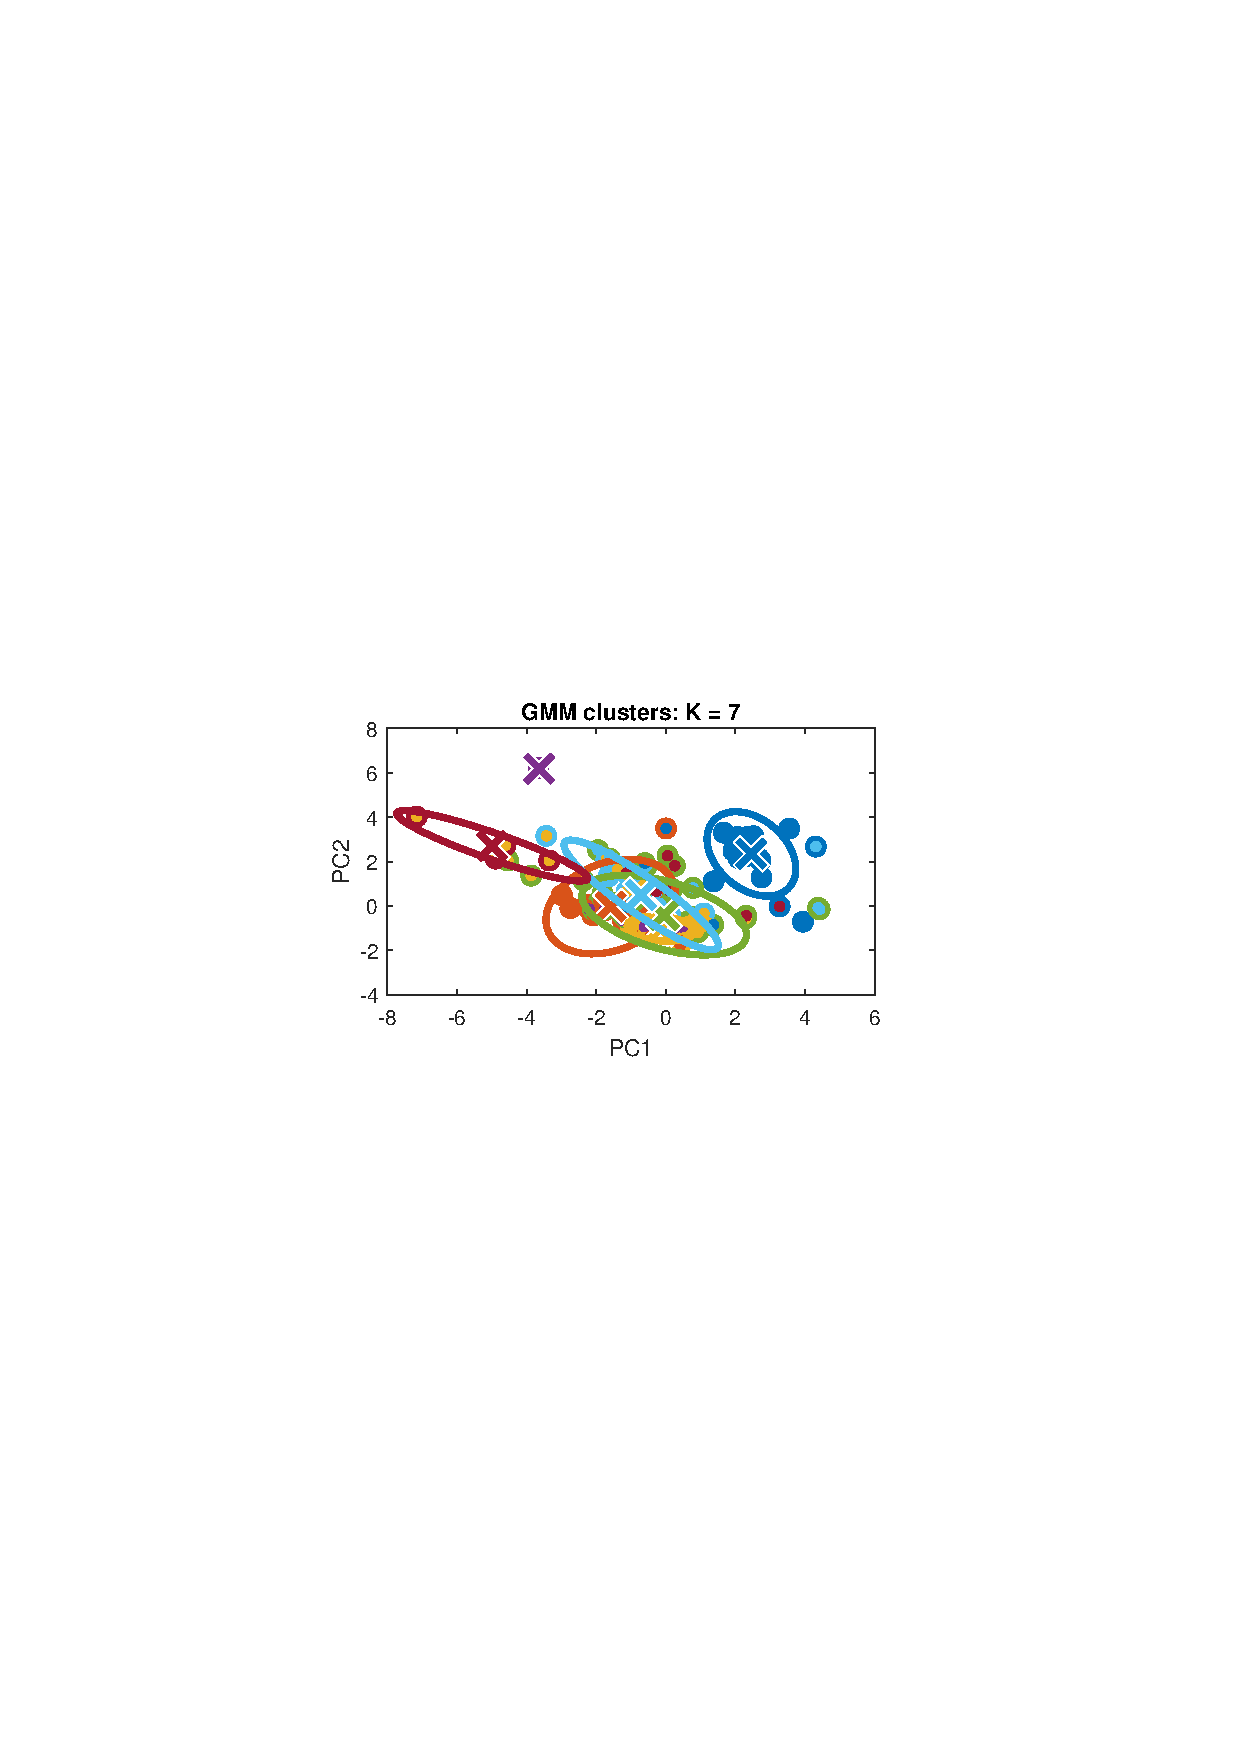
\includegraphics[width=0.45\textwidth]{fig/GMM_clusters_7_twofig.pdf}
    \caption{GMM plot for $K = 7$ clusters.}
    \label{fig:GMM_clusters_7}
\end{figure}

\begin{figure}[H]
    \centering
    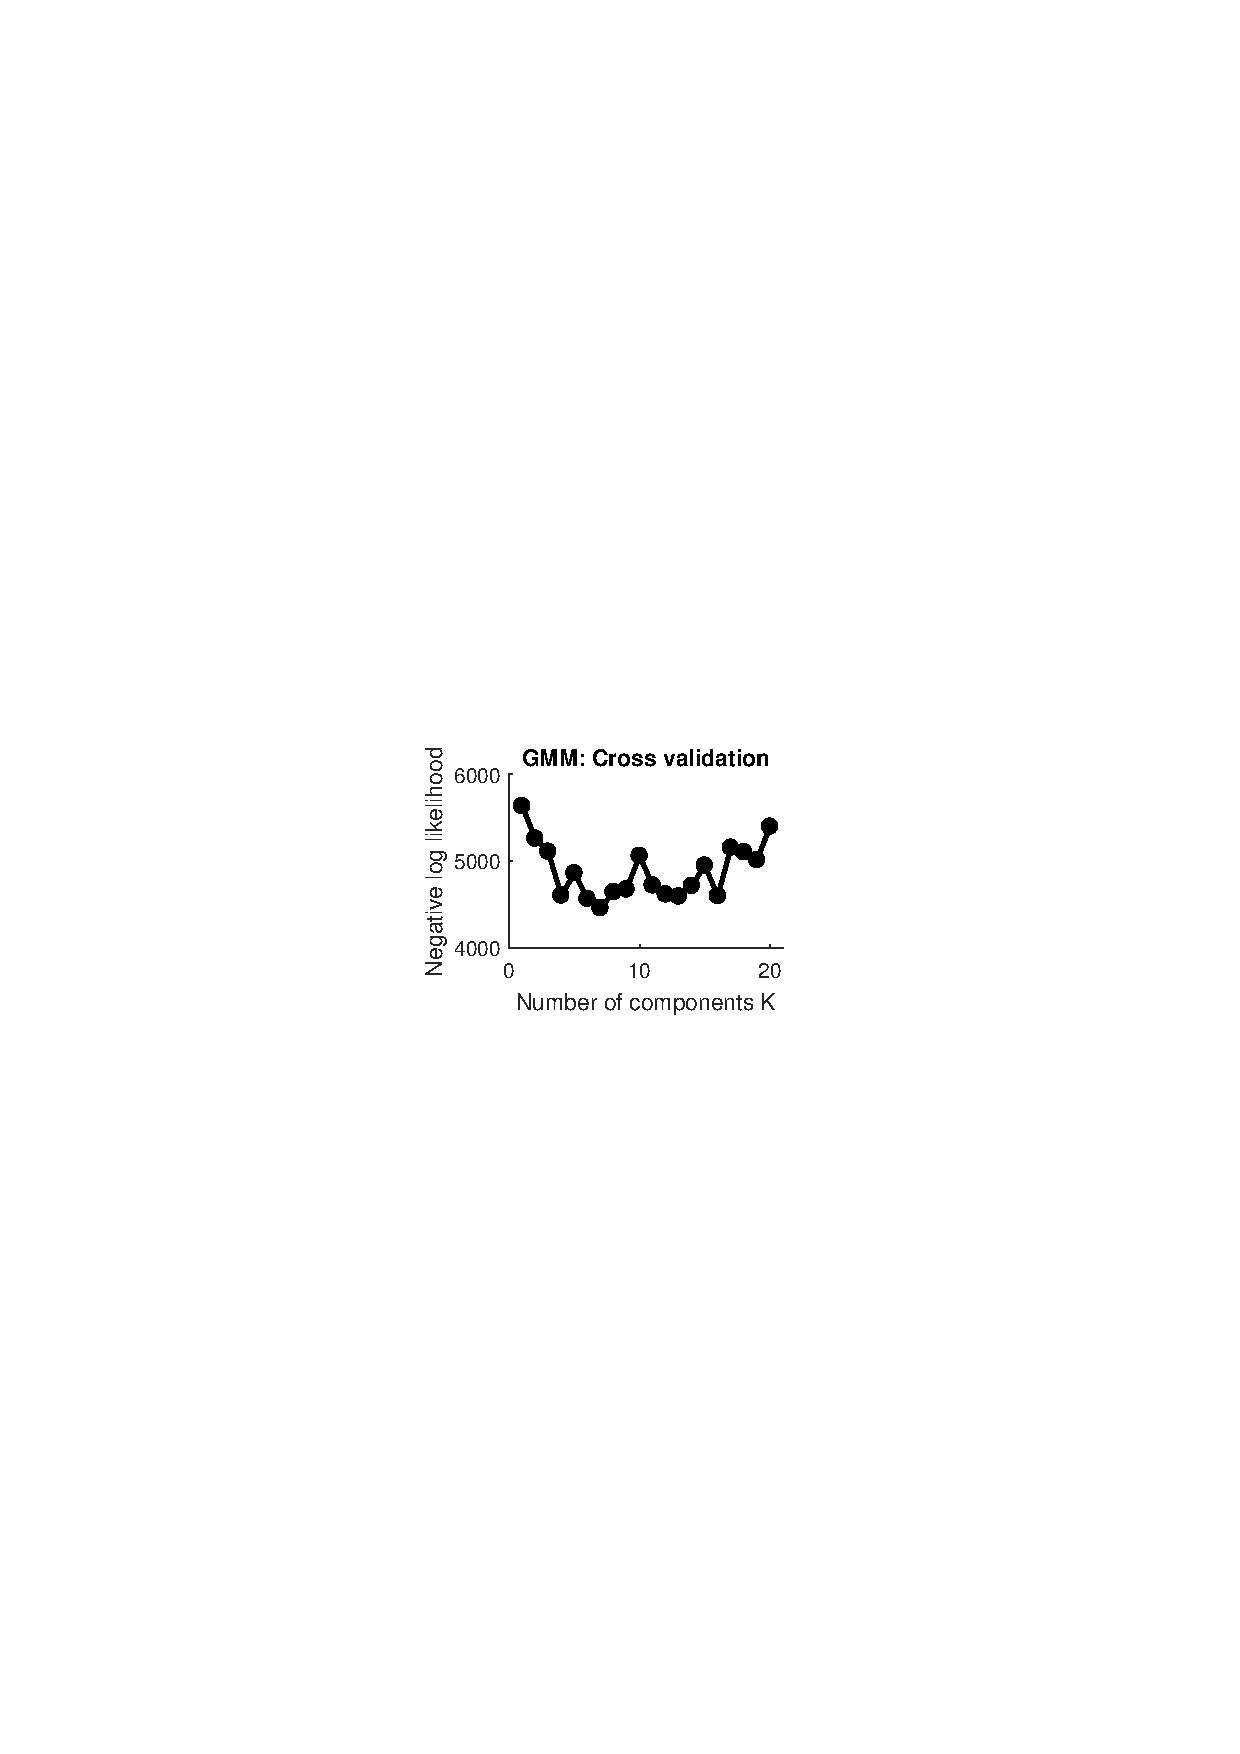
\includegraphics[width=0.30\textwidth]{fig/GMM_number_of_components_reg_twofig.pdf}
    \caption{Cross validation error as estimated negative log likelihood. The minimum occurs at $K = 7$.}
    \label{fig:GMM_number_of_components}
\end{figure}
\end{multicols}


\textbf{Interpreting extracted centers:} The unsupervised learning method GMM found 7 clusters. We want to investigate whether the clusters correspond to the "true" classes from the supervised learning problem in report 2. It is difficult to determine from inspecting the plot (Fig \ref{fig:GMM_clusters_7}) only. In report 1, we found that the first two components of the PCA analysis accounted for only $\approx$ 50 \% of the variation, and 5 principal components were needed to account for 90 \% of the variation. As we found in report 1, the "areas" covered by each glass type on the PCA plot overlapped a lot. The purple "cluster" consists of one data point only, so this is likely an outlier, and will be further explored in the report section on outliers.

By comparing the GMM plot with $K=7$ with the original PCA plot from report 1, we learn that the dark blue centroid in Fig \ref{fig:GMM_clusters_7}  corresponds to glass type 7: headlamp. So the GMM method performs well if the problem is to identify whether a fragment of glass is from a headlamp which may have been worn by, say, a burglar. Since the glass identification problem is tied to crime-scene investigations, this is good news!

